%\documentclass[conference]{IEEEtran}
\documentclass[10pt,conference]{IEEEtran}
\IEEEoverridecommandlockouts
% The preceding line is only needed to identify funding in the first footnote. If that is unneeded, please comment it out.
\usepackage{cite}
\usepackage{amsmath,amssymb,amsfonts}
\usepackage{algorithmic}
\usepackage{graphicx}
\usepackage{textcomp}
\usepackage{xcolor}
\usepackage{url}
\usepackage{listings}
\usepackage{courier}
\usepackage{xspace}
\usepackage{multirow}
\usepackage{colortbl}
\usepackage{blindtext}

%\newcommand{\sd}[1]{\textbf{"\textsc{SD:}} \textit{#1}"}

\newcommand{\nnbb}[2]{
    \fbox{\bfseries\sffamily\scriptsize#1}
    {\sf\small$\blacktriangleright$\textit{#2}$\blacktriangleleft$}
   }
\newcommand{\sd}[1]{\nnbb{\textcolor{orange}{St\'{e}f}}{\textcolor{orange}{#1}\xspace}}
\newcommand{\hr}[1]{\nnbb{Henrique}{#1\xspace}}
\newcommand{\ap}[1]{\nnbb{\textcolor{blue}{Apierr}}{\textcolor{blue}{#1}\xspace}}
\newcommand{\Miner}[0]{Miner\xspace}
\newcommand{\Miners}[0]{Miners\xspace}
\newcommand{\miner}[0]{miner\xspace}
\newcommand{\miners}[0]{miners\xspace}
\newcommand{\gas}[0]{gas\xspace}
\newcommand{\Gas}[0]{Gas\xspace}
\newcommand{\Transaction}[0]{Transaction\xspace}

\newcommand{\SmartGas }[0]{\textsc{SmartGas}\xspace}

\newcommand{\eg}{\emph{e.g.,}\xspace}
\newcommand{\ie}{\emph{i.e.,}\xspace}
\newcommand{\etal}{\emph{et al.,}\xspace}
\newcommand{\ct}[1]{{\textsf{#1}}\xspace}
\usepackage[scaled=0.85]{helvet}

\def\BibTeX{{\rm B\kern-.05em{\sc i\kern-.025em b}\kern-.08em
    T\kern-.1667em\lower.7ex\hbox{E}\kern-.125emX}}
\begin{document}

\title{Toward  maintainance of  a commencial software: Defects model }
% \title{Toward  maintainance of  a commencial software: Time serie model of defects }
%\thanks{Identify applicable funding agency here. If none, delete this.}}

\author{\IEEEauthorblockN{HOUEKPETODJI Mahugnon Honore\IEEEauthorrefmark{1}\IEEEauthorrefmark{2},
Nicolas Anquetil\IEEEauthorrefmark{3}}
\IEEEauthorblockA{\IEEEauthorrefmark{1}University of Lille, France}
\IEEEauthorblockA{\IEEEauthorrefmark{2}Inria Lille - Nord Europe, France}
homahugnon@gmail.com, nicolas.anquetil@inria.fr}


\maketitle

\begin{abstract}
Legacy systems are old software that style does useful tasks. In industrial software companies, legacy systems are often crucial for the company business model and represent a longterm business investment. Legacy systems are known to be hard to maintain. This is the case in a french company whose main product is twenty years old software written in PowerBuilder (we call it SPB).  Our longterm goal is to help reengineer. But how to validate our intervention? Using moving average, and regression, we evaluate the maintenance state of SPB and produce a dashboard to monitor our future actions. We validate our results with the developer team. We  In this paper, we present a lightweight defects model to help planning commercial software maintenance
\end{abstract}

\begin{IEEEkeywords}
Lagacy system, Defect model .
\end{IEEEkeywords}

\section{Introduction}
Software companies usually invest time and energy to improve the quality of the software they develop to respond to the rising market demands. Features are developed in a hurry sometimes.  As results, they less allow resources for software refactoring to remove source code defects.   As the software is out of control and it becomes hard to improve or maintain. Rewriting this software require time and a lot of resources. At this point, one of the solutions is to reverse-engineer them.  


The main business product is SPB of our company. Our longterm goal is to reverse-engineer SPB.  With over 3,000,000 lines of codes, continually updated for more than 20 years,  SPB is not versioned and not unit tested. Bugs is registered in a database without correlation with which part of the system is responsible for the bug. Old versions of SPB are lost until 2012. The original developers of SPB are part of the developers' team. So the currents developers only know SPB partially.  So we could not completely rely on developers view of the system. Besides, there is also a misunderstanding between developer team and the business team. As the business team doesn't know the state of SPB.  In this condition, it is completely impossible to successfully reengineer SPB without  15 years of the useful data model and our analytics.


Our data model and analytics have to the main goal. It provides a report on the state of SPB to the entire company and shows the business team the need to reengineer  SPB. Furthermore, it will help us to monitor our future task on SPB.  In this paper, we will present the data model and the analytics we made.


This paper is structured as follow: 


\section{Related Work}\label{sec:related-work}

\section{Background}\label{sec:background}
\subsection{Presentation of SPB}
SPB is build with PowerBuilder. PowerBuilder is an enterprise development tool that allows you to build many types of applications and components. A powerBuilder application components are grouped by libraries.   A PowerBuilder library contains differents type of Objects: Datawindow, User object, Global function, etc.    In SPB libraries  can be grouped by business module . Figure  \ref{fig:pbArchitecture} give an overview of SPB achitecture.
\begin{figure*}[!ht]
    \centering
    {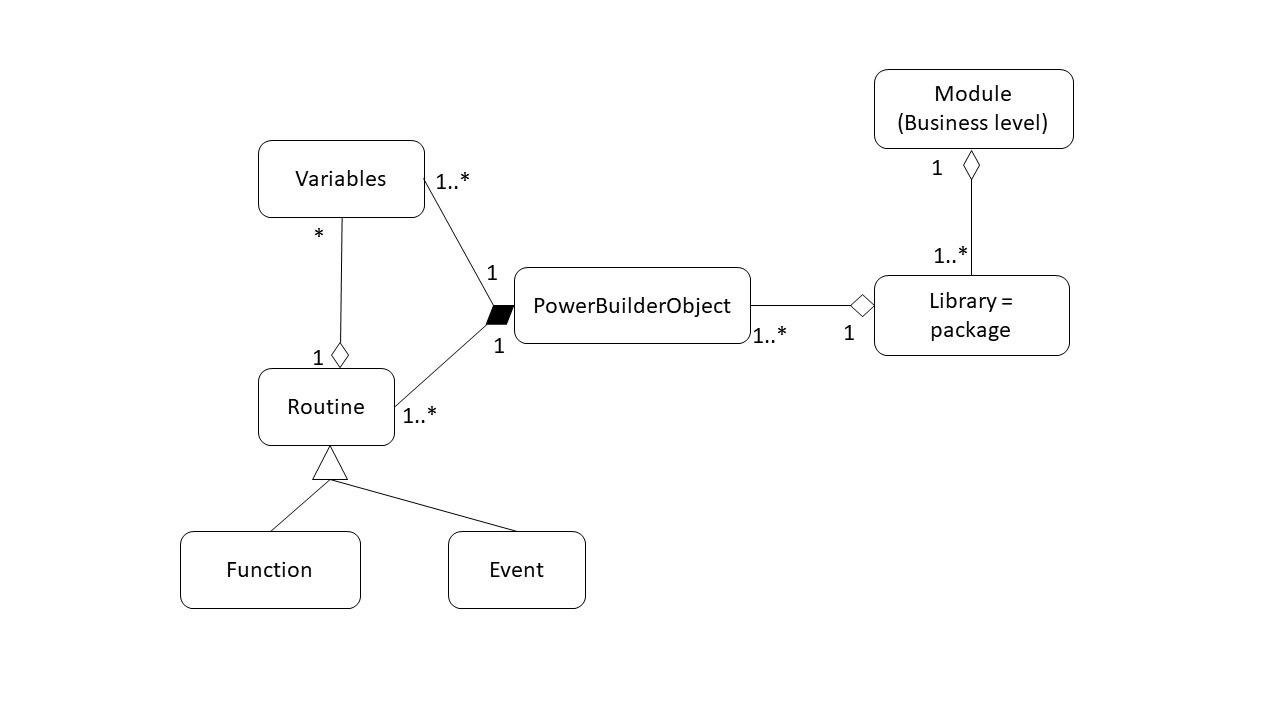
\includegraphics[width=0.9\linewidth]{images/pbArchitecture.jpg}}
    \caption{Simplified SPB achitecture.
Very simplified architecture of SPB}\label{fig:pbArchitecture}
 \end{figure*} 
\subsection{Ticket}
A ticket is related do a task to do.  This task can be fixing a bug, writing documentation, adding a new feature, etc.  A ticket is open for a task . Once the task is done and validated, the ticket is close. A ticket has the following characteristics:
\begin{itemize}
\item the libraries it  is related to
\item the creation date
\item the closing date
\item time spent by a developer
\begin{itemize}
\item time to analyze
\item time to implement solution
\item time to test
\end{itemize}
\item  the estimation of the time needed by the developer to work on the ticket
\end{itemize}

\section{Methodology}\label{sec:methodology}
We collected data  from the company Tickets database .  Then we procced to data cleaning.
The data analytics process is guided by the following research rule:
\begin{itemize}
\item Pose problem
\item Make experimentations on data
\item Validation of results
\end{itemize}
\subsection{Data collection and data cleaning}
The ticket database contains data from 1998  until 2019.  This data includes tickets  differents teams and softwares in  the company. In the field related to the  library a ticket is related to,  the name of the library is not always well written. 

  The  datas are consistent  from 2004 to 2019 . We  remove all tickets, non related  to SPB and reformat durations per ticket. By inteviewing developers, we categorize tickets into to sets: tickets related to defects and tickets related two evolutions.

 \subsection{Problems}
 \begin{itemize}
 \item  Is  there a correlation between defects and evolutions per libraries:
 \begin{itemize}
 \item Does evolutions cause defect?
 \item  Does evolutions occur after defects occur?
 \end{itemize}
 \item Is there a relationship between defects  and libraries:
 \begin{itemize}
 \item Does defects in a librarie cause defect in other libraries?
 \item Does some libraries always have defects together?
 \end{itemize}
 \item How long in average does it take to open and close a ticket?
 \item How long in average  does a developer spend on a ticket ?
 \item How long in average does a developer spend to test a ticket after development ?
 \item Does the team manager estimate well  the time needed by the developer?
 \item If the time estimated by the team manager is good, does the developer finish because  of time constraint?
 \end{itemize}
 
 \subsection{Experimentations}
For each problem, we experiement on the ticket database. 
 \subsubsection{Correlation between defects }
We plot  defects and evolution per library over time.  In x axis we have years and in y axis  we have the number of defects  or evolutions.  According to  the visualizations, some libraries trends to as many defects as  evolution over time. For some libraries, we observe that they do not have defects. Some others seem to  have defects after evolution. 
 \section{Results and Discussion}\label{sec:results-discussion}


  
\section{Summary and Conclusions}\label{sec:conclusion}

%\bibliographystyle{IEEEtran}
\bibliographystyle{alpha}
\bibliography{rmod,others,new}

\vspace{12pt}
\end{document}
